\chapter{Augmenting Predicate Analysis with Invariants}
Before this master's thesis, invariants were used in \CPAchecker{} only for \Kinduction{} and path invariants\,\sidenote{Path invariants are a \PredicateCPA{} specific feature.}. The 
implementation of path invariants was not complete and had issues related to the problems with the \texttt{CPAInvariantGenerator} and \texttt{InvariantSupplier} as stated in 
\autoref{title:arch_old}. In the following, we describe the various options for utilizing invariants for enhancing the \PredicateCPA{}. First, we focus on locations where invariants
can be added, then, new approaches to invariant generation are described. In the last section of this chapter, we introduce a generalized handling of invariants for the \PredicateCPA{}.

\section{Invariant Injection Strategies}
In \autoref{title:predicatecpa} the \PredicateCPA{} was introduced. Its states consist of two formulas, a path formula $\phi$ and an abstraction formula $\psi$. Additionally, each state has a 
precision $\pi$, which consists of predicates that are used to compute the abstraction formula at abstraction locations specified by the $\blk{}$ operator. The three components, precision,
path formula, and abstraction formula, 
are potential candidates for adding invariants. The following sections provide more detailed insights on the advantages and drawbacks of adding (potentially-) invariant
formulas\,\sidenote{Differences in formula encoding (mainly due to pointers, or variables not tracked in the consumer analysis) may lead to having potentially invariant formulas instead of definite 
invariants.} to each of these parts.


\subsection{Using Invariants as Precision Increment}\label{title:inv_prec}
The precision $\pi$ of the \PredicateCPA{} contains predicates that are used for computing the abstraction formula during precision adjustment. During a normal analysis, the precision is 
initially empty, and predicates are added in the refinement step of the \ac{CEGAR} algorithm (cf. \autoref{alg:CEGAR}). The new predicates, called precision increment, are usually computed by 
interpolation, but they can also be generated in other ways, for example by heuristically mining them from the \ac{CFA}\,\sidenote{Assume statements could, \eg, be used as predicates.}. In this approach, we add 
invariants as precision increment. This is the safest way of using potentially-invariant formulas compared to the other two injection options, as it is not important that the 
added formula actually is an invariant for the running analysis. When computing the new abstraction formula $\psi' = (\phi \land \psi)^\pi$ with the precision $\pi$ we can use arbitrary predicates  
$p_i$ as precision 
objects\,\sidenote{We do also need a propositional variable $v_i$ for each $p_i$, cf. \autoref{title:predicatecpa}.}. These predicates are only part of the new abstraction formula if $\phi \land \psi 
\land \bigwedge_{p_i \in \pi}(p_i \iff v_i)$ has satisfying assignments containing the predicates. Thus, adding invalid predicates to the precision has no negative effect on the accuracy of the analysis. 
Overall, adding invariants as predicates to the precision is safe, but comes with the drawback that performance may suffer, as the all-sat computation becomes more expensive with growing 
size of the precision. The performance drawback depends on the used invariants: if they are strong enough to refute the counterexample found with \ac{CEGAR} without further predicates, then 
the performance should not be differing much from only using interpolation, as the size of the precision does not increase more than it would be increasing by doing interpolation.

\subsection{Appending Invariants to the Path Formula}
The path formula $\phi$ is computed in the transfer relation of the \PredicateCPA{} by using the strongest post operator $\mathtt{SP}_{op}$ such that the successor abstract state $e' = (\psi', 
\phi')$ for an abstract state $e = (\psi, \phi)$ and a \ac{CFA} edge $g = (l, op, l')$ is given by $\phi' = \mathtt{SP}_{op}(\phi)$ and $\psi' = \psi$. During precision adjustment, if a block 
abstraction should be done, the path formula is reset to \true{} and the abstraction formula is computed. Conjoining an invariant $inv$ to the path formula before computing the abstraction results 
in the formula $\psi' = (\phi \land \psi \land inv)^\pi$ due to the associativity of the logical and.
Due to the immediate abstraction the invariant has only a very small chance of affecting the analysis. Therefore, we also conjoin the invariant to the new path formula after the abstraction\,\sidenote{
The necessity of this step is explained later on in the example in \autoref{title:combiningInv}.}. Thus, instead of resetting the path formula to \true{} we reset it to the invariant in this case.
This implies that the conjoined formula needs to be an invariant, a potential invariant is not enough, as otherwise we create an incorrect formula. An obviously incorrect example is to add \false{} as 
invariant, which makes the whole formula \false{}, and therefore leads to wrong results for the analysis. In contrast to that, adding \true{}, which is always an invariant, does not change the abstraction 
computation, just as intended. As stated in the introduction of this section, we do not have drastically wrong invariants such as \false{}, but there may be some encoding issues\,\sidenote{Path invariants 
are also not applicable here, this is discussed in \autoref{title:sharingReached}.}. In the evaluation, we will see that in most cases, it is safe to use the invariants generated by \CPAchecker{} for 
appending it to the path formula, too. Additionally, this approach doesn't have the performance drawback that may result from incrementing the precision with invariants.


\subsection{Appending Invariants to the Abstraction Formula}
Lastly, we can append computed invariants to the abstraction formula directly $\psi' = (\phi \land \psi)^\pi \land inv$. In this approach, it is critical that the conjoined formula is an invariant. 
There is no filtering of invalid predicates, and also no abstraction of the path formula that abstract from potentially invalid formulas such that we still have valid formulas afterwards\,\sidenote{Adding non-invariant formulas to the path formula is still unsound, but might not be noticed due to the described effect.}. If we 
are sure that we have invariants, this is the approach that is the least detrimental for performance, as neither the size of the path formula nor the size of the precision increases, both of which might 
have negative impact on the performance of the satisfiability query used for the abstraction.

\subsection{Combining Invariant Use-Cases}\label{title:combiningInv}
The approaches on utilizing invariants in the \PredicateCPA{} introduced in the last three sections can also be combined. For example, appending invariants to the path formula is not helpful if
the precision does not contain the necessary predicates. By adding an invariant to the path formula and the precision, we can therefore increase the accuracy of the analysis. In the following we 
will show the differences on an example.

\begin{figure}
 \centering
 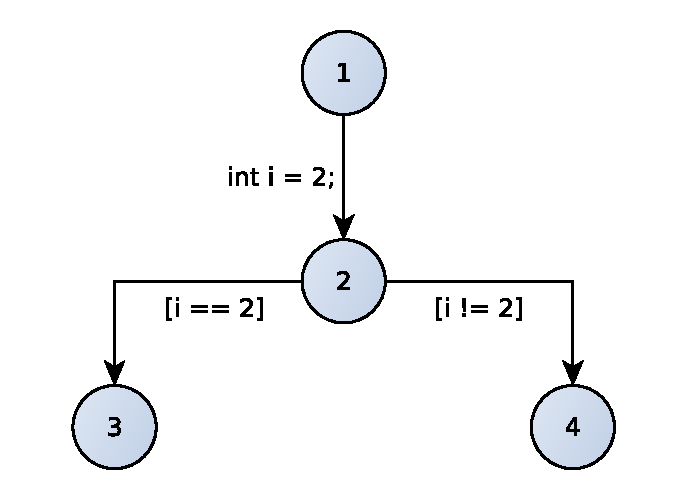
\includegraphics[width=.5\textwidth]{../graphics/inv_usage_example}
 \caption{A \acs{CFA} for illustrating the usage of invariants}
 \label{fig:inv_usage_example}
\end{figure}

Consider the control flow shown in \autoref{fig:inv_usage_example}, the global precision $\pi = \{ i < 10 \}$ and the location invariant $i = 2$ for location 2. $\blk{}$ considers locations in front of
conditions as being abstraction locations. We start with the state $e_0 = (\text{\true{}}, \text{\true{}})$ and compute the strongest postcondition for the path formula for the transition of location 1 to 2, the successor 
is then given by $e_1 = (\text{\true{}}, i = 2)$. Location 2 is right before two assume edges, and according to $\blk{}$ we treat it as the end of a block. Thus, we have to compute the abstraction before 
continuing. Now we have several options: we can refrain from using invariants at all (\textbf{No Inv}), we can add the invariants to the precision (\textbf{Prec}), we can append them to the path or 
abstraction formulas (\textbf{PF}, \textbf{AF}), or any combination of these. 

\begin{table}
\centering
 \caption{Differences in using invariants at different locations in the \PredicateCPA{}}
 \label{table:inv_usage_example}
\begin{adjustbox}{max width=\textwidth}
 \begin{tabular}{lrll}
 \toprule
  Strategy & \multicolumn{2}{c}{New Abstract State} & Possible Transitions\\
  \midrule
  No Inv& $(i < 10$,& $\text{\true{}})$ & $2 \rightarrow 3$, $2 \rightarrow 4$\\
  Prec & $(i = 2 \land i < 10$,& $\text{\true{}})$ & $2 \rightarrow 3$\\
  PF & $(i < 10$,& $i = 2)$ & $2 \rightarrow 3$\\
  AF & $(i < 10 \land i = 2$,& $\text{\true{}})$ & $2 \rightarrow 3$\\
  Prec + PF & $(i = 2 \land i < 10$,& $i = 2)$ & $2 \rightarrow 3$\\
  Prec + AF & $(i = 2 \land i < 10 \land i = 2$,& $\text{\true{}})$ & $2 \rightarrow 3$\\
  PF + AF & $(i < 10 \land i = 2$,& $i = 2)$ & $2 \rightarrow 3$\\
  Prec + PF + AF & $(i = 2 \land i < 10 \land i = 2$,& $i = 2)$ & $2 \rightarrow 3$\\
  \bottomrule
 \end{tabular}
 \end{adjustbox}
\end{table}

\autoref{table:inv_usage_example} shows the different strategies, the path formula and the abstraction formula \emph{after} the abstraction, and the feasible transitions in the \ac{CFA}. By 
simplifying the given formulas, some predicates could be omitted, but this is an expensive task for the \ac{SMT} solvers, so we do not simplify them here to show the potential redundancy caused by 
using invariants.
What can be seen is that any of the previously described invariant-usage approaches is sufficient to prevent the analysis from taking an invalid transition. For \textbf{PF}, this is only the 
case because we use the invariant as the new path formula instead of \true{}. Otherwise, the information that $i = 2$ would be lost due to the coarse precision, and the analysis would behave as if 
no invariants are used. Additionally, it does not make sense to use combinations of one of these approaches with \textbf{AF}, because this always results in duplicate clauses in the new formula.
In  case of \textbf{PF + AF} this is not obvious, because the duplicate formula will only come at the next abstraction, when the old abstraction already contains the invariant, and the path formula which 
gets conjoined to the abstraction formula does also contain it. In contrast to \textbf{PF + AF}, the combination of adding invariants to the precision and conjoining them to the path formula makes sense, 
otherwise one cannot be sure that the invariant conjoined to the path formula provides any benefit, because the precision might be too coarse. Using this combination is close to \textbf{AF} as it is very 
likely that the invariant predicate from the precision holds and is therefore used in the abstraction formula afterwards, this can also be seen in \autoref{table:inv_usage_example}, the only difference 
is that for $Prec + PF$ the new path formula starts with the invariant instead of \true{}.

Overall, the approaches \textbf{Prec}, \textbf{PF}, \textbf{Prec + PF} and \textbf{AF} seem to be most promising, where \textbf{PF} should be worse than \textbf{Prec + PF} due to the issues discussed in 
the last paragraph. \textbf{Prec} is the best option when only potentially-invariant formulas are used. For the other approaches, we need to be sure that we have real invariants. In the evaluation, we 
will have a look at all possible combinations of invariant usage strategies and compare their performance.

\section{New Invariant Generation Approaches}
In \autoref{title:concept} the generalization of asynchronous invariant generation was introduced. In this section we explain all invariant generation approaches that are used later on in the 
evaluation. All of them are implemented in \CPAchecker{} and do not rely on external invariant generators. The approaches are divided into three parts: first we focus on invariants computed out 
of reached sets. Second we move on to sharing precisions. The third part consists of lightweight invariant-generation heuristics that are tied to the usage of the \PredicateCPA{}.

\subsection{Sharing Finished Reached Sets}\label{title:sharingReached}
By generalizing the idea of continuously-refined asynchronous invariant generation in \autoref{title:architecture_final}, we now have the possibility to use finished reached sets not only from $\mathtt{CPAInvariantGenerator}$ for 
invariant generation. For example, we can have a sequential combination of analyses where the first analysis is very coarse. Due to infeasible counterexamples, we can not use the result of this 
analysis, but we can use its reached set for generating invariants for the next analysis, such that some of the computational effort of the first analysis was not completely wasted. By combining 
analyses with different strengths this way, we might be able to prove safety of programs where it would not be provable otherwise.
With parallel analyses, reached sets can only be exchanged in a meaningful way, if one of the parallel analyses is continuously refined\,\sidenote{Even running a fast analysis in parallel, which is not 
continuously refined, does not make much sense. This analysis could then simply be used in a sequential combination and provide the computed reached set already at the beginning to the consumer analysis.}, 
such that we have a quickly terminating analysis whose reached set can be provided to the other running analyses. Both approaches will be analyzed exhaustively in the evaluation.

A special case, neither completely sequential nor parallel, are path invariants. They are computed sequentially, not before the consumer analysis is executed, but in between instead. Path 
invariants~\cite{Beyer:PathInvariants} for the \PredicateCPA{} were introduced in \CPAchecker{} as part of a 
seminar work. They suffered from encoding problems described in \autoref{title:arch_old} but this was not recognized, because path invariants can only be used as precision increment (cf. 
\autoref{background:pathinvariants}. For this thesis, path invariants were rewritten and integrated with the other invariant generation approaches. For generation of path invariants we run an analysis 
restricted to the counterexample path inside the current analysis via the \texttt{CPAInvariantGenerator}. Afterwards, the invariants are retrieved location-wise and used as precision increment.


While sharing reached sets is a generic approach that can be used by any analysis, some additional code is necessary such that an other analysis can take advantage of the given reached sets. For 
the \PredicateCPA{} it is important that the invariants are \ac{SMT} formulas. Creating an \ac{SMT} formula out of a state in a reached set is not implemented for all \acp{CPA} available in \CPAchecker{}. Thus we are restricted to the analyses working on states we can use, which are those, implementing the interface \texttt{FormulaReportingState} in \CPAchecker{}.
By using the \texttt{FormulaInvariantsSupplier} introduced in \autoref{title:concept_reached} we can then obtain invariants out of reached sets containing states of this kind.


\subsection{Sharing Precisions}
For sequential combinations of analyses, we do not only have the possibility to use the reached set of the earlier analyses in the later ones, but we can also dump the precision of the earlier 
analysis and use this precision in later analyses. This is, however, bound to certain \acp{CPA} as the precision is a \ac{CPA}-specific object. Still, a fast primary analysis discovering some initial 
predicates for a later, slower but more precise, analysis could make sense. This approach does not rely on having real invariants, but it is related to adding invariants to the precision as described 
in \autoref{title:inv_prec}.


\subsection{Lightweight Heuristics}\label{title:lightweightHeuristics}
In this section we focus on invariant generation via heuristics. These heuristics are not guaranteed to find invariants, so their applicability greatly depends on the computational overhead they 
have in case no invariants are found. For this thesis, three different heuristics were invented which are described in the following paragraphs.

\paragraph{Checking Interpolants with $k$-Induction}
Slicing an infeasible counterexample path into distinct --- still infeasible --- path prefixes and then selecting the prefix which should be used for refinement is a technique to guide the
refinement~\cite{Beyer:RefinementSelection}. We do not select one prefix out of the computed prefixes, but instead we take all of them and check each on $1$-inductivity with \Kinduction{}. The
non-determinism of the \ac{SMT} solver allows us to compute even more prefixes by creating interpolants more often for the same formula. The amount of unique interpolants found depends on the amount of 
possible solutions, so we chose to have three interpolation runs for the same formula as default. This number can be changed via a configuration option. The invariants discovered this way, can then be
used to either increment the precision or conjoining them to the path formula or to the abstraction formula.

\paragraph{Inductive Weakening of Path Formulas}
Formula slicing is a technique for finding an invariant by weakening a given loop precondition based on the effects of the loop transitions~\cite{Karpenkov:Slicing}. The weakening process is guided by 
counterexamples-to-induction by an \ac{SMT} solver. This approach is implemented in \CPAchecker{}. A complete analysis configuration is available with the name \emph{formula-slicing}. We use this 
technique as a blackbox and provide the necessary input: the path formula before the loop start and the loop transitions. The result when using this blackbox is an invariant which we can use. In 
the worst case, the invariant is simply \true{}, so besides additional runtime we have no bad side-effects and the generated invariants can be used to either increment the precision, or conjoining 
them to the path or abstraction formula.


\paragraph{Checking Conjuncts of Path Formulas on Inductivity}
Equally to weakening the path formula by removing clauses until the formula is inductive, we have added a heuristic that at first transforms the path formula into \ac{CNF}\,\sidenote{Our 
\ac{CNF} conversion tool does support to not create a full \ac{CNF} but to only have it on higher levels such that the exponential explosion of this transformation can be omitted.} and then splits 
the formula into its conjuncts. The conjuncts are separately checked on $1$-inductivity with \Kinduction{}. The invariants discovered this way, can then be used to either increment the precision, or 
appending them to the path or abstraction formula.


\section{Generalized Invariants handling in the \mbox{\PredicateCPA{}}}
In the last sections several different invariant generation and usage strategies for the \PredicateCPA{} were introduced. To simplify usage and provide a clean interface, all invariant generation 
approaches are centralized in the class \texttt{PredicateCPAInvariantsManager} (cf.~\autoref{fig:inv_manager}). 

This class aims at providing all necessary features and hiding all invariant-generation related details. It does also handle
the computation of invariants from reached sets of other analyses. The generation of invariants is strictly separated from the retrieval of invariants in order to increase the performance. In 
earlier implementations, invariants for a certain location were generated lazily as soon as they were requested. However, this is not possible for all invariant generation strategies we have. 
Additionally, when considering conjoining invariants to the path formula or the abstraction formula during precision adjustment, this happens very often, and thus takes a lot of time\,\sidenote{Abstractions are computed as indicated by $\blk$, this is usually much more often than, \eg, refinements are computed.}.

Our solution is to switch from the lazy generation approach to a more eager one: Now invariants are computed during refinement. The reasons for this solution are:
\begin{itemize}
 \item the usually small amount of refinements, leading to few invariant generations but also guiding invariant generation to the important locations of the program\,\sidenote{Computing invariants for program locations not leading to an error takes time that does not need to be spent.}, and
 \item the availability of information necessary for invariant computation, for example path invariants can only be computed during refinement as they need an infeasible counterexample path and information about the contained loops.
\end{itemize}

\begin{figure}
 \centering
 \includegraphics[width=\textwidth]{../graphics/inv_manager_arch.png}
 \caption{Managing invariants in the \PredicateCPA{}}
 \label{fig:inv_manager}
\end{figure}

The following two sections provide detailed information about invariant generation and its usage.

\subsection{Invariant Generation}
Invariant generation in the \PredicateCPA{} is split into three parts. First, we have the invariants computed out of reached sets of other, concurrently or sequentially running, analyses (we call 
them global invariants here), and at second, we have the invariants computed by the heuristics mentioned in the previous sections. The third part are path invariants which are handled separately 
from the other invariant-generation approaches as their invariants cannot be used for conjoining them to the path or abstraction formula. The methods described in the following paragraph can also be 
seen in \autoref{fig:inv_manager}.

Global invariants do not need further computation besides taking the reached sets and conjoining all states per location. Thus, updating them is easy and can be done by calling 
\texttt{updateGlobalInvariants}. This method is necessary to avoid changes to the global invariants between several invariant retrievals, for example, when retrieving invariants for adding them to 
precisions along an infeasible counterexample path, we want the invariants to come from the same reached set(s), and not from different ones. Due to the probably concurrently added new reached sets we 
need to decouple the updates on stored reached sets in the \AggregatedReachedSets{} object from the reached sets used for invariant generation.

For locally computing invariants with one or more of the mentioned heuristics, the method \texttt{findInvariants} has to be called. There are several configuration options for this:
\begin{itemize}
 \item The heuristics that should be used can be specified as a list, with the option \emph{cpa.predicate.invariants.generationStrategy}.
 \item The heuristics in the list are executed in the given order, either until a heuristic succeeds in generating an invariant, or if all given heuristics should be used depending on 	
  the configuration option \emph{cpa.predicate.invariants.useAllStrategies}.
 \item A time limit for invariant generation can be given with the option \emph{cpa.predicate.invariants.timeForInvariantGeneration}.
 \item Besides the mentioned options there may also be separate options for each of the heuristics such as the analysis that should be used for the generation of path invariants.
\end{itemize}
Invariants generated in this way are cached for later usage, subsequent calls of \texttt{findInvariants} resulting in different invariants do not replace earlier results but are conjoined to them.

In contrast to that, path invariants can only be generated and retrieved at once, with the method \texttt{findPathInvariants}. Because they only hold for the specific given path, they are not cached but 
can only be used directly for the path they were generated for.

\subsection{Invariant Retrieval}
Retrieving invariants is done via the method \texttt{getInvariantFor}, receiving a location and the necessary information about pointer aliasing\,\sidenote{Variables that are aliased by pointers are 
encoded in a special way, this encoding has to be added to the generated invariants.} as input. Depending on the configuration, invariants 
are retrieved from other reached sets (if available) and conjoined to the locally computed invariants by a heuristic. Calling \texttt{getInvariantFor} several times in a row for the same location 
and with the same pointer aliasing information is guaranteed to return the same invariants if none of the invariant-generation methods introduced in the last section were called in the meantime. 
For also having the information about the usage strategies available and configurable at one location in the \PredicateCPA{} and not spread over several classes, we added the methods 
\texttt{appendToAbstractionFormula}, \texttt{addToPrecision}, and \texttt{appendToPathFormula}  which indicate if invariants should be used for the given purpose.